% !TeX root = ../main.tex
% Add the above to each chapter to make compiling the PDF easier in some editors.


\chapter{Implementation}\label{chapter:Implementation}
The subsequent chapter is going to give a detailed view of how the methods described in section \ref{chapter:Concept}, were implemented. Moreover, possible problems regarding the process are listed. 
As the Android-application described in passage \ref{chapter:Integration into existing App} was used as a basis, there is no reasonable alternative to further developing the app with Android Studio.

\section{Target device}
As target device, the mid-range phone Huawei P8 Lite ALE-L21 is going to be used (Figure: \ref{fig:p8lite}), with the phone specifications seen in Table \ref{table:specifications}.
\begin{table}[h]
	\begin{tabular}{|p{0.3\linewidth} || p{0.58\linewidth}|}
		\hline
		\multicolumn{2}{|c|}{Relevant specifications} \\
		\hline\hline
		CPU & Hisilicon Kirin 620 CPU 8 X 1.2 GHz \\
		\hline
		GPU & ARM Mali-450MP4 \\
		\hline
		Operating System & Android 6.0  \\
		\hline
		Memory & 2 GB RAM + 16 GB ROM \\
		\hline
		Connectivity & LTE Cat4/ Wi-Fi 802.11 b/g/n/ Bluetooth 4.0/ \\
		\hline
		Camera & 13 MP BSI camera + 5 MP camera\\
		\hline
		Video & 1080p@30fps \\
		\hline
	\end{tabular}
	\caption{Specifications}
	\label{table:specifications}
\end{table}
\begin{figure}[h]
	\centering
	\minipage{0.35\textwidth}
	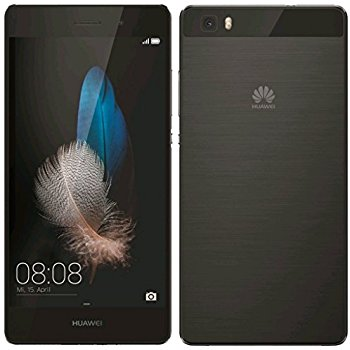
\includegraphics[width=\linewidth]{images/p8lite.jpg}
	\caption{Huawei P8 Lite ALE-L21}\label{fig:p8lite}
	\endminipage\hfill
\end{figure}

\section{Native Development Kit}
The Android NDK is a toolset that lets you implement parts of your app in native code, using languages such as C and C++. For certain types of apps, this can help to reuse code libraries written in those languages \cite{androidndk}. Moreover employing the Native Development Kit to the application's code can increase the performance significantly  \cite{ndkspeed}. Anticipated using the Native Kit might have a bigger workload, than Android's classic SDK, was considered just fine, if the performance was superiorly compared to the approach written in Java. \newline
The first part, dealing with the detection of Speed Signs, doing image processing with OpenCV,  was relatively simple in C++, compared to the mammoth task of building Tensorflow from source, loading a model and integrating everything into the actual app. It actually was so time-consuming, it looked like it could not be done on schedule. A lack of supporting features like code completion and code correction in Android Studio, poor documentation from Tensorflow (at least for novices to the framework) paired with proportionally sparse discussion board entries on "Stack Overflow", that often referenced different versions, led to the turning point, where the NDK was given up for the SDK. In total, this excursion cost about one to two weeks of time, that had been reserved for the implementation. 

\section{Extracting Speed Sign Candidates}\label{extraction}
The algorithm has been implemented in three languages: C++, Java and Python, every language serving different purposes. C++ and Java versions were necessary to operate for the application, first one running the Native approach, the second for the "standard" SDK version. The last program written in Python has been utilized for extracting data from images collected from Google image search, running on PC, in order to get training data to feed my Neural Network model (more about this topic later on). Nevertheless, apart from syntactical differences, every program basically does the same operations. For the sake of simplicity, only the python variation is going to be examined, as it is probably the easiest version to read. Every step of image processing in every language has been done with the OpenCV library. \newline
After reading the image, changing the colour space from RGB/BGR to HSL/HSV is optional, but a reasonable step, because in the RGB/BGR space, all three Values of red, green and blue are correlated when it comes to changes in brightness \cite{imagesegmentation}. Unlike that, HSL/HSV holds lightness or the value of brightness in a separate variable, which can lead to better results with respect to filtering colours under alternating lighting conditions. In the following, the HSV space is going to be used, even though HSL space is defined almost analogical, they differentiate each other from the arrangement of white color \cite{zynq}. \newline

\begin{figure}[H]
	\centering
	\minipage{0.5\textwidth}
	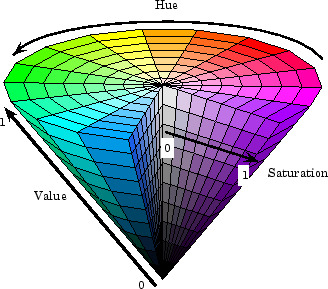
\includegraphics[width=\linewidth]{images/hsv.jpg}
	\caption{HSV colourspace \cite{hsv}}\label{fig:hsv}
	\endminipage\hfill
\end{figure}


Nevertheless filtering red pixels from our preferred colourspace works slightly different than just excerpting the Red channel of an image, as it would be done using RGB:
%\begin{figure}[H]
%	\minipage{\textwidth}
%	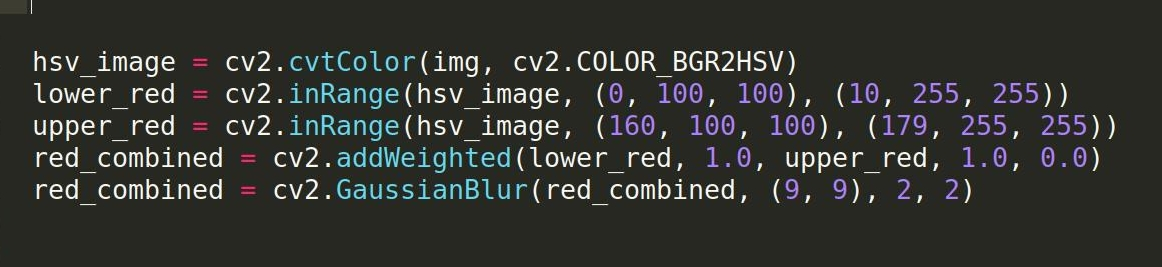
\includegraphics[width=\linewidth]{images/filterredimage.jpg}
%	\caption{Python code for extracting red pixels}\label{fig:filter_red_code}
%	\endminipage\hfill
%\end{figure}


\lstset{style=custompy}
\begin{minipage}{\linewidth}
\begin{lstlisting}[language=python]
hsv_image = cv2.cvtColor(img, cv2.COLOR_BGR2HSV)
lower_red = cv2.inRange(hsv_image, (0, 100, 100), (10, 255, 255))
upper_red = cv2.inRange(hsv_image, (160, 100, 100), (179, 255, 255))
red_combined = cv2.addWeighted(lower_red, 1.0, upper_red, 1.0, 0.0)
red_combined = cv2.GaussianBlur(red_combined, (9, 9), 2, 2)
\end{lstlisting}
\end{minipage}

At first ranges of HSV values have been extracted, that are considered to be red. This is done in two slices, for the upper range (Figure: \ref{fig:lower_red}), and one for the lower (Figure: \ref{fig:upper_red}). After these two slices are combined into one single binary image (Figure: \ref{fig:combined}), the Gaussian Blur filter is executed (Figure: \ref{fig:combined_blurred}) on the image, to prepare it for the Circle Hough transform, in order to avoid false positive circles.\newline
 
%\begin{figure}[H]
%	\minipage{\textwidth}
%	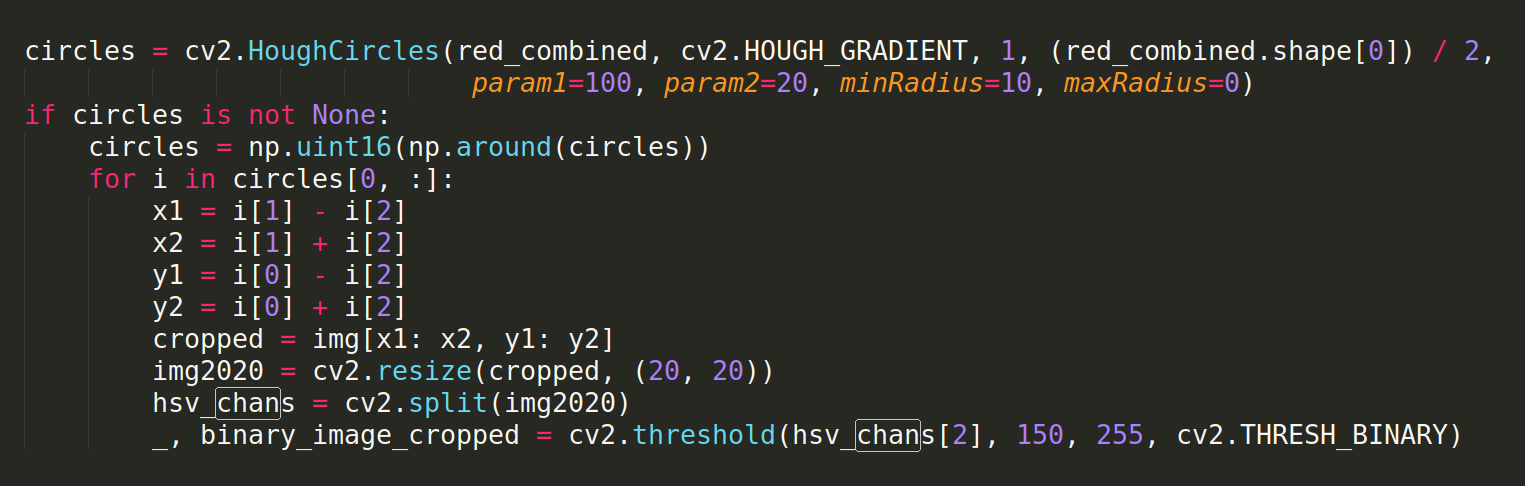
\includegraphics[width=\linewidth]{images/detectioncode.png}
%	\caption{Code for performing Circle Hough Transform}\label{fig:detection_code}
%	\endminipage\hfill
%\end{figure}

\begin{minipage}{\linewidth}
\begin{lstlisting}[language=python]
circles = cv2.HoughCircles(red_combined, cv2.HOUGH_GRADIENT, 1, (red_combined.shape[0]) / 2, param1=100, param2=20, minRadius=10, maxRadius=0)
if circles is not None:
	circles = np.uint16(np.around(circles))
	for i in circles[0, :]:
		x1 = i[1] - i[2]
		x2 = i[1] + i[2]
		y1 = i[0] - i[2]
		y2 = i[0] + i[2]
		cropped = img[x1: x2, y1: y2]
		img2020 = cv2.resize(cropped, (20, 20))
		hsv_chans = cv2.split(img2020)
		_, binary_image_cropped = cv2.threshold(hsv_chans[2], 150, 255, cv2.THRESH_BINARY)
\end{lstlisting}
\end{minipage}

When executing the HoughCircles Function \cite{houghcircles}, the result is passed to the circles variable, this function returns all found circles, described with an array of [x-coordinate, y-coordinate, radius],  after checking whether any circles were found, these values only have to be rounded to integer. Looping  over the array containing triplets, delivers every found circle. \newline
In order to crop the input image, the x- and y- coordinates of the cropping window are being calculated, this window can be described by the coordinates of two edges. After actually cropping the image this section is resized to the desired 20 by 20 pixels format (Figure: \ref{fig:2020}). Then this sub picture is converted from coloured to binary format (Figure: \ref{fig:2020bin}). Now the image is actually ready, to be passed to the Neural Network. It should be noted, there can be multiple candidates in one image that need to be passed further.   

\begin{figure}[H]
	\minipage[t]{0.33\textwidth}%
	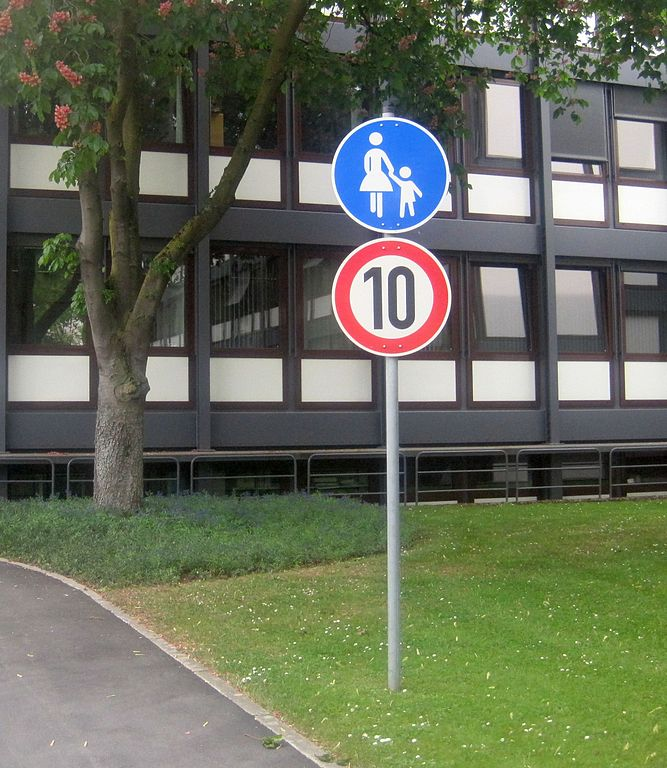
\includegraphics[width=\linewidth]{images/101.jpg}
	
	\caption{Original Image}\label{fig:original_image}
	\endminipage\hfill
	\minipage[t]{0.33\textwidth}
	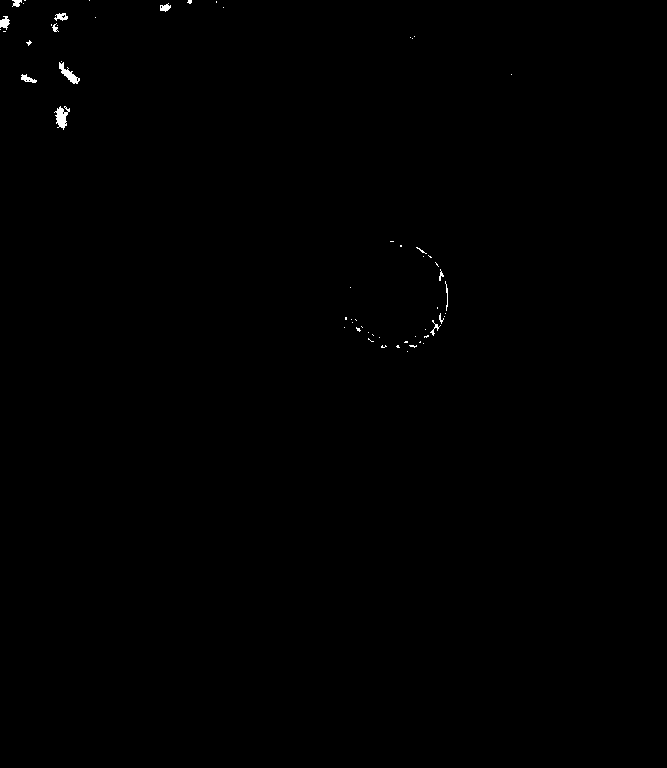
\includegraphics[width=\linewidth]{images/lowerred.png}
	\caption{Lower red hue pixels}\label{fig:lower_red}
	\endminipage\hfill
	\minipage[t]{0.33\textwidth}%
	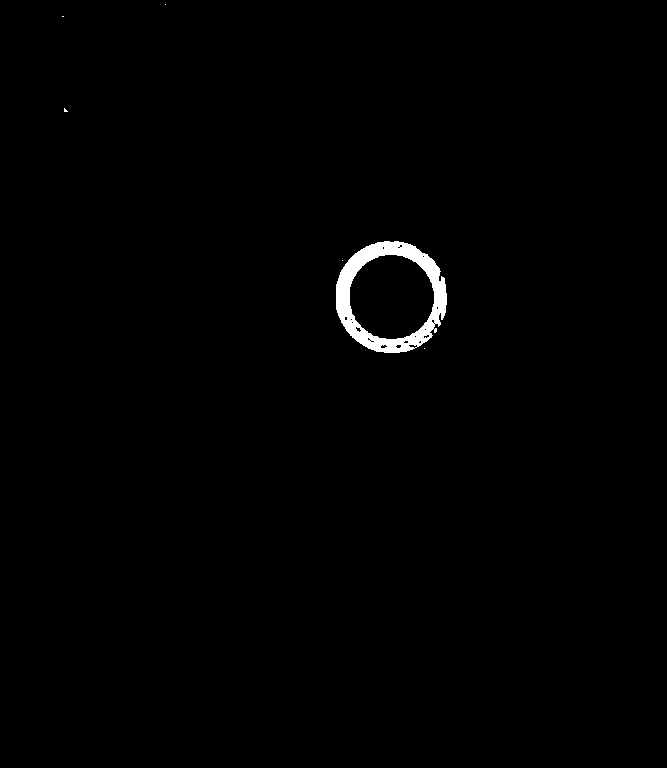
\includegraphics[width=\linewidth]{images/upperred.png}
	\caption{Upper red hue pixels}\label{fig:upper_red}
	\endminipage\hfill
	\newline
	\newline
	\minipage[t]{0.33\textwidth}
	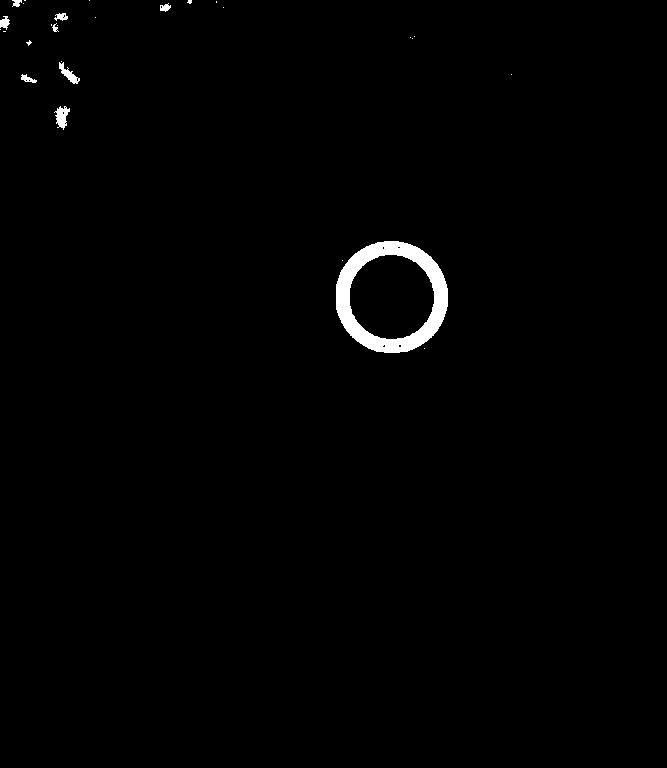
\includegraphics[width=\linewidth]{images/redcombined1.png}
	\caption{Upper and lower pixels combined}\label{fig:combined}
	\endminipage\hfill
	\minipage[t]{0.33\textwidth}
	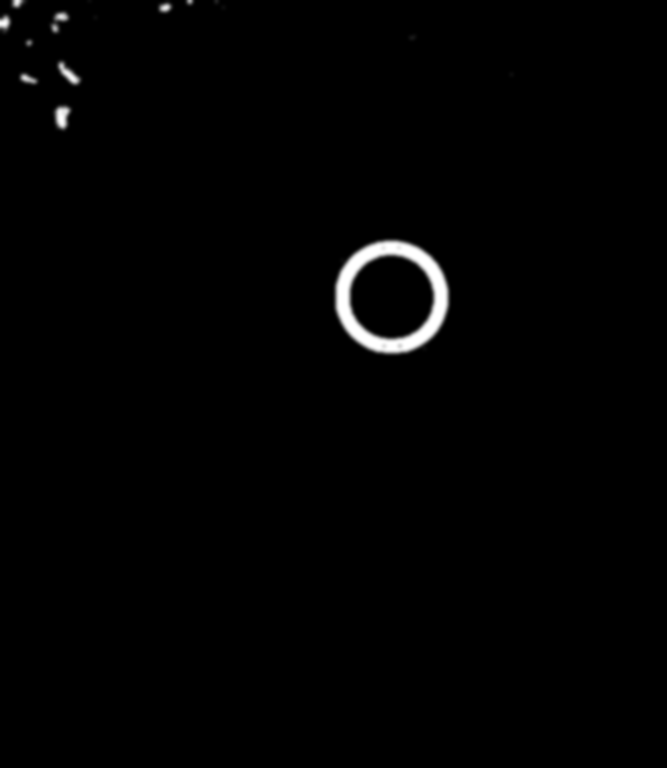
\includegraphics[width=\linewidth]{images/redcombined2.png}
	\caption{Gaussian Blurred}\label{fig:combined_blurred}
	\endminipage\hfill
	\minipage[t]{0.33\textwidth}
	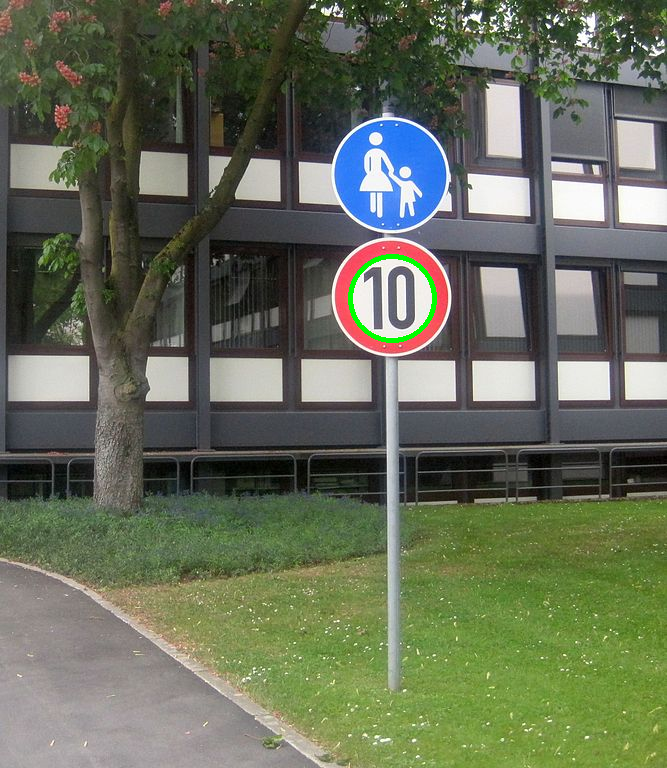
\includegraphics[width=\linewidth]{images/detectedcirclescircle.png}
	\caption{Marked circle in original image}\label{fig:detectedcircles}
	\endminipage
	
\end{figure}

\begin{figure}[H]
	\minipage[t]{0.49\textwidth}%
	
\includegraphics[width=\linewidth]{images/2020.png}
	\caption{Cropped image}\label{fig:2020}
	\endminipage\hfill
	\minipage[t]{0.49\textwidth}%
	
\includegraphics[width=\linewidth]{images/binaryimg.png}
	\caption{Cropped and converted image}\label{fig:2020bin}
	\endminipage\hfill
	\newline
	
\end{figure}

\section{Neural Net Classification}
Hypothetically speaking, above excerpt image(s) only needs to be filled into a tensor, fed into the model and subsequent the result(s) need to be fetched. Though, getting to this point, there needs to be done several work, regarding the Neural Network.  

\subsection{Building Neural Network with Tensorflow}
TensorFlow™ is an open source software library for numerical computation using data flow graphs. Nodes in the graph represent mathematical operations, while the graph edges represent the multidimensional data arrays (tensors) communicated between them. \cite{tensorflow} When it comes to building models on a PC, Tensorflow's C++, Go, Java or Python API could be used, although the core is programmed in C++ \cite{tensorflowcore}. It was decided to use the Python API for the project, because again this language was considered to be the easiest choice. \newline

% \begin{figure}[H]
%	\centering
%	\minipage{\textwidth}
%	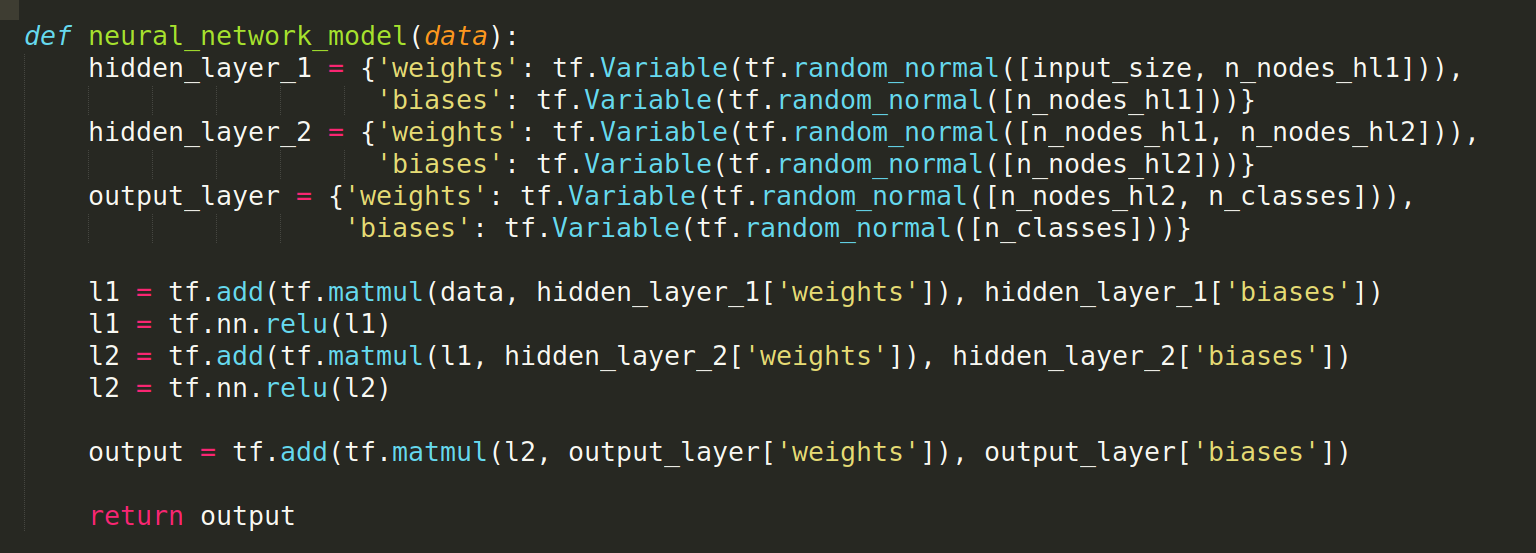
\includegraphics[width=\linewidth]{images/neuralnetmodelcode.png}
%	\caption{Neural Net Model in Python}\label{fig:NNmodelPyth}
%	\endminipage\hfill
%\end{figure}
\begin{minipage}{\linewidth}
\begin{lstlisting}[language=python]
def neural_network_model(data):
	hidden_layer_1 = {'weights': tf.Variable(tf.random_normal([input_size, n_nodes_hl1])), 'biases': tf.Variable(tf.random_normal([n_nodes_hl1]))}
	hidden_layer_2 = {'weights': tf.Variable(tf.random_normal([n_nodes_hl1, n_nodes_hl2])), 'biases': tf.Variable(tf.random_normal([n_nodes_hl2]))}
	output_layer = {'weights': tf.Variable(tf.random_normal([n_nodes_hl2, n_classes])), 'biases': tf.Variable(tf.random_normal([n_classes]))}
	
	l1 = tf.add(tf.matmul(data, hidden_layer_1['weights']),hidden_layer_1['biases'])
	l1 = tf.nn.relu(l1)
	l2 = tf.add(tf.matmul(l1, hidden_layer_2['weights']), hidden_layer_2['biases'])
	l2 = tf.nn.relu(l2)
	
	output = tf.add(tf.matmul(l2, output_layer['weights']), output_layer['biases'])
	
	return output
\end{lstlisting}
\end{minipage}

Obviously, the "data" parameter, given to the neural\_network\_model represents the input tensor, thus it holds every pixel provided by the image. The dictionaries "hidden\_layer\_1", "hidden\_layer\_2" and "output\_layer" hold the weights and biases of the incoming edges, they are all initialized with random values before the training phase. The "tf.add" and "tf.mul" adds, respectively multiplies two tensors. The variables "l1" and "l2" each have two initialization steps, in the first, preceding nodes are multiplied with the corresponding weights and added to it's biases. The second part calls "tf.nn.relu", which is just the activation function used for this network. The "output" variable after all holds and returns the final output tensor. 

\subsection{Preparing training data}
\subsubsection{Collect images}
As the Artificial Neural Network uses some data, to be trained in order to run correctly, a certain amount of data was needed. Searching for a suitable dataset did not bring the expected results, so it was necessary to create a training dataset. The focus has been set to the scope from 10km/h to 90km/h, so for each individual sign, Google image searches were performed manually, with search terms like "x km/h sign", "tempo x", "speed limit x", ...  To avoid false positive detections, i also searched for some signs with red edges, that did not represent speed limits. A folder, called "images" was created, that contained more folders named: "10", "20", ..., "90", "nosign". For the processed images, a new folder was created called "cropped", containing sub folders ranging from "10" over "90" to "nosign". Described search led to a total of 219 images. 


\subsubsection{Process images}
Cropping every number manually would not have been too efficient, also not necessarily precise, so a Python script was written, having the core functionality described in section \ref{extraction}, with the extension of traversing every folder hold by the "image" directory, executing the algorithm and finally saving the resulting image sections into the "cropped" directory to the corresponding folder. At last an inspection of the results had to be done by hand, since the algorithm from \ref{extraction} searches for red circles, at least some false positives could be expected. Examining the freshly filled folders, every image not containing proper values of speed signs was cut and pasted to the "nosign" folder, frames containing numbers, but badly displayed were deleted to prevent the Network from being trained in the wrong direction. In total, 222 images could be used for further training. Additionally the amount of processed pictures was separated into training and validation data, to check whether the ANN works correctly. Overall 39 images were selected to operated as test data, remaining 183 were actually used in order to practice. 

\subsubsection{Creating TfRecord file}
There are diverse mechanics to import data, for training purposes, but the recommended technique is to use a TFRecord file \cite{tensorflowdata} that holds the image's data, including the encoded pixel values, labels, names or in fact every meta data needed or wanted. To give an idea of what a TFRecord file looks like inside, an extraction of the training data has been provided in Listing: \ref{lst:tfrecord}. There can be seen a TFRecord file containing one image that is labeled as 80, it should also be noted, the "image/encoded" value has been shortened, to consume less space in this listing, in fact in the real file, this part is considerably longer.\newline 
As mentioned before, two different data sets were demanded. So with the help of a little script, that basically traverses every sub folder of a given folder, encodes and adds every image and it's inherent meta data to the TFRecord. After processing every wanted image, the resulting TFRecord file is being saved and can now be used for further steps of feeding it's held data into a NN. 

\begin{minipage}{\linewidth}
\begin{lstlisting}[language=python, caption={Minimized Excerpt of a  TFRecord file}, label={lst:tfrecord},captionpos=b]
features {
	feature {
		key: "image/class/label"
		value {
			int64_list {
			value: 8
			}
		}
	}
	feature {
		key: "image/class/text"
		value {
			bytes_list {
			value: "80"
			}
		}
	}
	feature {
		key: "image/encoded"
		value {
			bytes_list {
			value: "\377\330\377\340\000\020JFIF\000\001\001\...
			...\241|I\0231\216EGVE\373>\212+\377\331"
			}
		}
	}
	feature {
		key: "image/filename"
			value {
			bytes_list {
			value: "815(0).jpg"
			}
		}
	}
}

\end{lstlisting}
\end{minipage}

\subsection{Tensorflow Sessions}
A Session object encapsulates the environment in which Operation objects are executed, and Tensor objects are evaluated\cite{tensorflowsession}. A session owns resources like Variables, in given case, all weights and biases are stored in a session, moreover if they change, say during the process of training, the current values are enclosed by the Session. In order to safe the current state of the graph, Tensorflow provides the Saver class, that allows easy saving of the whole session informations. 

\subsection{Feeding and training}


